\documentclass[12pt]{article}
\usepackage{amsmath,amssymb,amsthm}
\usepackage{graphicx,mathabx}
\usepackage{xcolor}
\usepackage{tikz}
\usepackage{placeins}
\usepackage{lipsum}
\usepackage[shortlabels]{enumitem}
\usepackage{placeins}
\usepackage[makeroom]{cancel}
\newcommand\tab[1][1cm]{\hspace*{#1}}
\begin{document}
\title{TCSS 343 - Week 4}
\author{Jake McKenzie}
\maketitle
\noindent\centerline{\textbf{Dynamic Programming}}\\\\\\\\\\\\\\\\
\begin{center}
    ``An optimal policy has the property that whatever the initial state and initial decision are, the remaining decisions must constitute an optimal policy with regard to the state resulting from the first decision." \\$\cdots$\\  Richard Bellman's \textbf{Principle of Optimality}
\end{center}
\begin{center}
    ``What we choose means more than what was handed to us by chance." \\$\cdots$\\  Ada Palmer
\end{center}
\begin{center}
    `` If `dynamic programming' didn't have such a cool name, it would be known as 'populating a table'". \\$\cdots$\\ Mark Dominus 
\end{center}
\newpage
\noindent 1. Today we're going to explore dynamic programming. Below are three implementations of the fibonacci algorithm that I wrote in python. I want you to draw the \textbf{``tree"} for each then reflect on how the ``bottom up" apprach is different from the other two? (Hint: They are all trees but also different types of trees. This is a key insight in my opinion in idea in understanding dynamic programming) \\
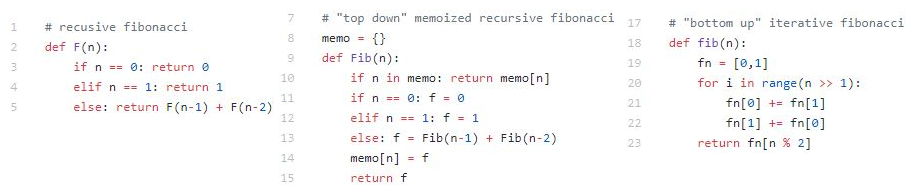
\includegraphics[width=\linewidth]{fib.jpg}
\newpage

\noindent 2. I found these really cool recursive Fibonacci formulas: 
$F_{2n+1}=F_{n+1}^{2}+F_{n}^{2}$ and $F_{2n}=2F_{n+1}F_{n}-F_{n}^2$
 now can you use them to find $F_{11}$ and $F_{10}$(worth noting that
 $F_2 = 1$, $F_1 = 1$, and $F_0 = 0$)?\\\\\\\\\\\\\\\\\\\\
 3. Can you now write an iterative method that computes $F_{2n}$ and $F_{2n+1}$
 using dynamic programming?\\\\\\\\\\\\\\\\\\\\\\\\\\\\\\\\\\\\\\\\
 4. How is this different from the basic Fibonacci formula? What is the
 time complexity of this function? Space complexity?
    \FloatBarrier
\newpage
\centerline{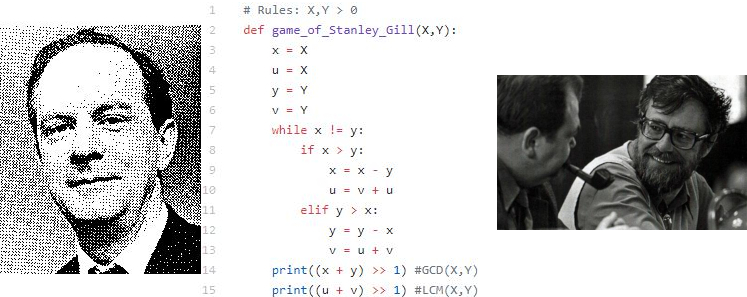
\includegraphics[scale = 2]{comb.jpg}}
\noindent 5. This is a game shown to Edsgar Dijkstra(pictured right) when he was still an undergraduate, attributed to Stanley Gill(pictured left), an early computer scientist. Now it is true that $2XY = xv+yu$, which can be seen when the variables are initialized. But is it always true given that $X,Y > 0$? Show why this is true. (Hint: You can use the comments to help you along. Remember that the $>> 1 $ operation is the same as $ / 2$.)
\newpage
\noindent 6. For the following problem stated as pseudo-code, let $A[\ell\dots r]$ denote the sublist of the integer list $A$ from the $\ell$-th to the $r$-th element inclusive, let \texttt{Cubic($A[1\dots n]$)} denote an algorithm that runs in time $\Theta(n^3)$.\\

{\ttfamily
$\phantom{A}$\\
$\phantom{---}$ Three($A[1\dots n]$)\\
$\phantom{--- ---}$ If $n \leq 1$ Then Return // nothing to do\\
$\phantom{--- ---}$ Cubic($A[1\dots n]$)\\
$\phantom{--- ---}$ Three($A[1\dots\lfloor\frac{n}{2}\rfloor]$)\\
$\phantom{--- ---}$ Three($A[\lfloor\frac{n}{4}\rfloor+1\dots \lfloor\frac{3n}{4}\rfloor]$)\\
$\phantom{--- ---}$ Three($A[\lfloor\frac{n}{2}\rfloor+1\dots n]$)\\
$\phantom{---}$ End Three.
}

\begin{enumerate}
\item [a.] State a recurrence that gives the complexity $T(n)$ for algorithm \texttt{Three}.

\item [b.] Find the tight complexity of algorithm \texttt{Three}.

\end{enumerate}
\newpage 
\noindent 7. For the following problem stated as pseudo-code, let $A[\ell\dots r]$ denote the sublist of the integer list $A$ from the $\ell$-th to the $r$-th element inclusive, let \texttt{Swift($A[1\dots n]$)} denote an algorithm that runs in time $\Theta(n\log(\log n))$.\\
{\ttfamily
$\phantom{A}$\\
$\phantom{---}$ One($A[1\dots n]$)\\
$\phantom{--- ---}$ If $n \leq 1$ Then Return // nothing to do\\
$\phantom{--- ---}$ Swift($A[1\dots n]$)\\
$\phantom{--- ---}$ One($A[1\dots\lfloor\frac{n}{2}\rfloor]$)\\
$\phantom{---}$ End One.
}

\begin{enumerate}
\item [a.] State a recurrence that gives the complexity $T(n)$ for algorithm \texttt{One}.

%\pagebreak

\item [b.] Find the tight complexity of algorithm \texttt{One}.

\end{enumerate}
\newpage
\noindent 8. The rod cutting problem has \textbf{overlapping subproblems} 
and \textbf{optimal substructure} which means we can solve it by dynamic programming.
\begin{enumerate}
    \item [a.] State a recurrence that gives the complexity $T(n)$ for the rod cutting problem.
    
    %\pagebreak
    
    \item [b.] State a tight asymptotic bound on the recursive solution to the rod cutting problem from $T(n)$ that you found.
    
    \end{enumerate}
\centerline{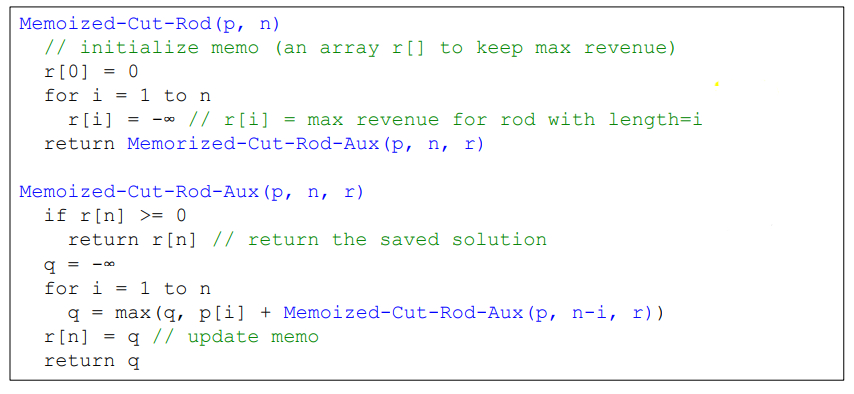
\includegraphics[scale = 2]{rodcutting.jpg}}
\newpage
\noindent 9. Say you have access to a function \textbf{dict} that returns true 
if its input is a valid English word, and false otherwise. We are given 
as input a sentence from which the punctuation has been
stripped (for example: ``dynamicprogrammingisfabulous"). 
Assuming calls to dict takes a unit time, give an $O(n^2)$ time 
algorithm to figure out whether an input string of length n can be
split into a sequence of valid words or not. 
HINT: Try to remove valid words from the end of the input string.
\newpage
\noindent \centerline{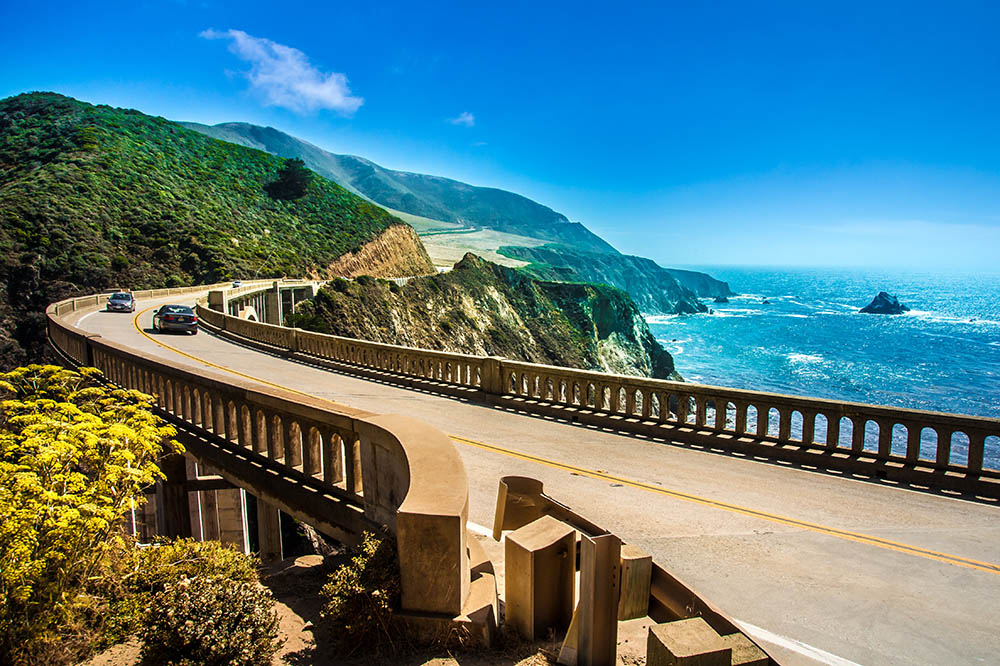
\includegraphics[scale = 1.25]{brix.jpg}}\\
A. So imagine you've graduated from University of Washington
in Tacoma and you got a nice job at a startup in San Francisco. It's the weekend
and you want to drive down to Monterrey to enjoy some wine with friends.
Now depending on what scenery you're driving through you find yourself
speeding through that locale for each time unit you're in it. It's the weekend
you don't really care how much time it takes you to get to Monterrey, but you
defintely don't want a ticket. What's the maximum amount of scenic value you can get
out of your weekend drive to Monterrey?

\begin{table}[]
    \begin{tabular}{|l|l|l|l|}
    \hline
    r & $sp_r$ & $sc_r$ \\ \hline
    1 & 5    & 1    \\ \hline
    2 & 9    & 6    \\ \hline
    3 & 26    & 18    \\ \hline
    4 & 31    & 22    \\ \hline
    5 & 36    & 28    \\ \hline
    \end{tabular}
    \end{table}
    \FloatBarrier
    \begin{table}[]
        \begin{tabular}{|l|l|l|l|l|l|l|l|l|l|l|l|l|l|l|l|l|l|l|}
        \hline
        r\textbackslash{}speedlimit & 0 & 5 & 10 & 15 & 20 & 25 & 30  & 35 & 40 & 45 & 50 & 55 & 60 & 65 & 70 & 75 \\ \hline
        \{1\}                  & 0 &   &   &   &   &   &    &   &   &   &    &    &    &    &    &  \\ \hline
        \{1,2\}                  & 0 &   &   &   &   &   &    &   &   &   &    &    &    &    &    &     \\ \hline
        \{1,2,3\}                  & 0 &   &   &   &   &   &    &   &   &   &    &    &    &    &    &    \\ \hline
        \{1,2,3,4\}                  & 0 &   &   &   &   &   &    &   &   &   &    &    &    &    &    &      \\ \hline
        \{1,2,3,4,5\}                  & 0 &   &   &   &   &   &    &   &   &   &    &    &    &    &    &     \\ \hline
        \end{tabular}
        \end{table}
        \FloatBarrier
\newpage
\noindent B. Let $s[1..m]$ and $t[1..n]$ be the two strings to be matched. 
Let $M(i,j)$ be the number of mismatches in the best alignment of $s[1..i]$ 
and $t[1..j]$. Which of the following is a correct recursive formulation 
of $M(i,j)$ for $i,j > 0$? Note: By convention $s[1..0]$ and $t[1..0]$ are taken 
to be the empty string, so $M(i, 0) = i$ for $i \in \{1,2,...,m\}$ and $M(0,j) = j$ 
for $j \in \{1,2,...,n\}$.\\\\
\begin{enumerate}[a)]
    \item $M(i,j) = 2+M(i-1,j-1)$, if $s[i]$ $\cancel{=}$ $t[j]$\\
    $min(M(i-1,j),M(i,j-1))$, otherwise
    \item $M(i,j) = M(i-1,j-1)$, if $s[i]$ $=$ $t[j]$\\
    $min(M(i-1,j),M(i,j-1))$, otherwise
    \item $M(i,j) = 1+M(i-1,j-1)$, if $s[i]$ $=$ $t[j]$\\
    $1+min(M(i-1,j),M(i,j-1))$, otherwise
    \item $M(i,j) = M(i-1,j-1)$, if $s[i]$ $=$ $t[j]$\\
    $1+min(M(i-1,j),M(i,j-1))$, otherwise
\end{enumerate}
C. You have a bag that you want to fill with toys. 
There are $N$ toys, and the ith toy has weight $w[i]$. The bag 
can hold a total weight of at most $W$. Maximize the number 
of toys you can take with you in the bag.\\\\
Formally, choose a set of as many toys as possible, 
such that the sum of their weights is $\leq W$.\\\\
Constraints: $N \leq 1000$; $w[i]$ $\leq$ $10,000$ $\forall$ $i$.\\\\
Choose the best option out of the following
\begin{enumerate}[a)]
    \item The simplest solution to this problem is using Dynamic Programming.
    \item This problem cannot be solved using Dynamic Programming.
    \item This problem can be solved with Dynamic Programming, but has a simpler solution without Dynamic Programming.
\end{enumerate}
\end{document}